
\begin{figure*}[tpb]
    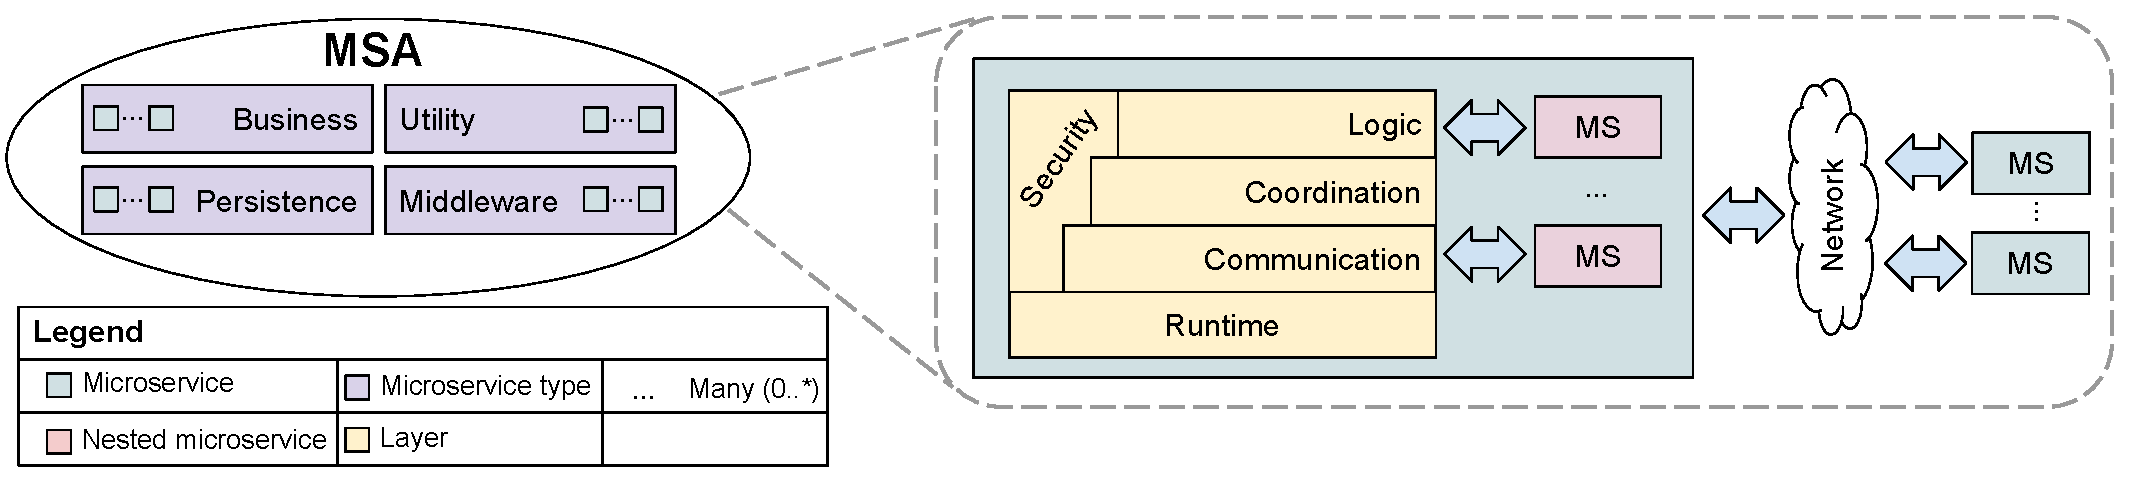
\includegraphics[scale=0.42]{images/msa-model.pdf}
    \caption{Generalized model of microservice architectures}
    \label{fig:model}
\end{figure*}

\section{Results}\label{sec:results}
\todo{In this section, the results of the literature review should be reported. This section can be split up according to the specific focus of the literature review, e.g. Publication Trends, Research Focus, and Potential for Industrial Adoption (see Running example)}

In this section we discuss the results of our literature review. The iterative model created from the selected studies is displayed in Figure~\ref{fig:model}. It defines the main components inside a microservice on an implementation level without detailing any topological specifics. Now the model is described.

\subsection{The Model}

There are four types of microservices, all of which are interconnected with other microservices through a network. (i) Business microservices implement logic towards a business objective, (ii) utility microservices facilitate business microservices with general functionality (e.g., logging, monitoring, circuit breakers, load balancers, service discovery, etc. \cite{richardson2018microservices}), (iii) persistence microservices typically provide database management systems (DBMS) or cache systems to business microservices, and finally (iv) middleware services which facilitate communication between other microservices (e.g., an API gateway, a message broker, a message bus, etc. \cite{richardson2018microservices,Garriga2018203}). An MSA is an interdependent cohesive loosely-coupled composition of these four types of services.

Every microservice can have nested microservices which only the parent microservice is allowed to communicate with. Nested microservices can be colocated on the same node as the parent microservice or hosted on separate nodes \cite{richardson2018microservices}. The former is generally the case with the sidecar pattern in which nested utility microservices are deployed to abstract away general functionality from the parent, while the latter is often the case with persistence services \cite{5-newman2021building,richardson2018microservices}.
A microservice consists of 3 layers with one overarching layer being security \cite{Garriga2018203,richardson2018microservices,Sill201676,5-newman2021building} and one foundational layer being runtime. Each layer is now described.

\textbf{Runtime} of a microservice consists of the platform on which it is executed. The industry has evolved such that physical hardware is abstracted away behind many layers of virtualization \cite{richardson2018microservices}. There are two levels of virtualization relevant to MSAs, (i) Hardware Abstraction Layer (HAL) virtualization (i.e., virtual machines \cite{richardson2018microservices}) and (ii) OS-level virtualization (i.e., containers \cite{Jaramillo2016,richardson2018microservices}). Microservices are typically deployed in either, or a combination, of these types of virtualized environment \cite{DiFrancesco201977}.

\textbf{Communication} between microservices consists of three parts \cite{Sill201676}, (i) the interaction model, (ii) the transportation and finally (iii) the presentation. The interaction model between services can be synchronous or asynchronous. Synchronous communication implies a request/response type pattern, meaning that it is vulnerable for services blocking other services while they are waiting for a response \cite{5-newman2021building, richardson2018microservices, IBMBook}. Asynchronous communication is non-blocking by definition and often comes hand in hand with event-based architectures \cite{Unlu2021244}. However, it requires state management within microservices and typically incurs more communication overhead due to it generally requiring some kind of middleware service, such as a message broker or message bus to facilitate and decouple message delivery \cite{richardson2018microservices, middleware, IBMBook}. Messages between microservices are transported either via the network or through Inter Process Communication (IPC) depending on performance and scalability requirements. The protocol used for transportation should be selected while considering the desired interaction model, since it can be performed using a variety of protocols \cite{Sill201676} (e.g., HTTP, gRPC, XMPP, MQTT, AMQP, etc.). Finally, presentation describes how the data is serialized such that it can be transported between services. Common serializers are JSON, XML and Protobuf \cite{richardson2018microservices}.

\textbf{Coordination} between services inside an MSA is necessary since it is a distributed system per definition \cite{5-newman2021building,richardson2018microservices, IBMBook}. The coordination within an MSA to perform more complex and elaborate functionalities are either choreography or orchestration based \cite{Garriga2018203,richardson2018microservices,4196179}. Orchestration requires composite services that directly coordinates with other services to oversee the process by receiving responses. On the other hand, choreography uses asynchronous events with the publish/subscribe pattern to facilitate collaboration \cite{Garriga2018203,richardson2018microservices,5-newman2021building}.

In essence, the coordination between microservices is about data management \cite{Laigner20213348}. There are  various challenges in data management all of which are subject of the next research question.

\textbf{Logic} is the last layer inside of microservices and includes all the programming required to implement the necessary functionality for each particular service. This can be anything due to our wide definition of microservices, ranging from business logic to DBMS logic. One important part of the logic layer is state management. Service can either be stateful or stateless \cite{IBMBook}. Statefulness implies session affinity, which in term means less flexibility and scalability \cite{7937885}. How and if state should be managed within a service can therefore be determined from the scalability requirements of that service.

\textbf{Security} is a layer that overarches all the previously defined layers and is challenging to implement properly. However, it vital within MSAs, due to the large attack surface and complicated connections between services \cite{shmeleva2020microservices}. There are two approaches to securing distributed systems, either a zero-trust-network or a trust-the-network approach \cite{christudas2019microservices,barth2017zero}. Depending on the security requirements of the MSA, a certain network type should be chosen \cite{shmeleva2020microservices,christudas2019microservices,Garriga2018203,barth2017zero}.

\subsection{Data Management}
The functionality of business microservices is commonly determined by applying domain-driven design (DDD) techniques \cite{evans2004domain}. In DDD, the problem space of the business is referred to as the domain. This domain can be divided into multiple subdomains each representing a different part of the business. Every subdomain has its own domain model, the scope of which is called a bounded context \cite{richardson2018microservices,Dragoni2017195,Unlu2021244,Santos2019145}. From this bounded context, one or more business microservices can be derived \cite{richardson2018microservices}. Typically, there is some (minimal) data dependency between the bounded context of these services. Therefore, inter-microservice data management (handled by the coordination layer in the model, Figure~\ref{fig:model}) is required, given that MSAs are commonly designed with a database per service pattern \cite{Soldani2018215}. According to the \textbf{CAP} theorem, any networked system which shares \textbf{P}artitions of data can only pick one of/attain a balance between the following two properties: \textbf{A}vailability or \textbf{C}onsistency \cite{6133253}. For example, a highly available MSA cannot be consistent all the time \cite{richardson2018microservices}. Therefore, depending on the consistency and availability requirements of the MSA, different solutions to facilitate inter-microservice data management are desirable. We now describe three common data management challenges found within MSAs.

\subsubsection{Inter-microservice data relations}\label{sec:foreign}
Consider two business microservices, one that keeps track of departments and one that keeps track of employees. Every department can have zero-to-many employees. In a relational DBMS, this type of relation is enforced by a foreign key on employee referring to the department of which the employee is a part of. The DBMS enforces policies to keep the database consistent, by for example, cascade deleting employees that are member of a deleted department, or making sure that every employee is member of a valid department. However, this type of enforcement is not trivial if each service has its own (possibly different type of) DBMS \cite{richardson2018microservices,5-newman2021building, Laigner20213348}. Foreign key emulation is currently resolved using ad-hoc implementations due to the lack of a general solution \cite{Laigner20213348}.

\subsubsection{Inter-microservice data transactions}
A transaction is a unit of work that needs to be completed in its entirety or rolled back. This is challenging to implement in MSAs due to the use of (polyglot) distributed persistence \cite{richardson2018microservices,IBMBook,Laigner20213348}. Consider two business microservices, $X_1$ that keeps track of inventory and $X_2$ that is responsible for the placement and tracking of orders. When an order is placed, the stock of the product is updated through the inventory service. A product with only one left in the stock is ordered by two users at the same time. Now $X_2$ receives two requests to check the stock followed by two requests to update the stock. A naive implementation allows the product to be ordered twice, since $X_1$ and $X_2$ do not coordinate the transaction. There are two solutions for this problem, depending on the desired properties of the MSA, displayed in Table~\ref{table:transactions}.

\textbf{Saga} is pattern in which eventual data consistency can be guaranteed by splitting up inter-microservice transactions into a sequence of compensable (potentially retryable) subtransactions each having the scope of only a single microservice \cite{richardson2018microservices,Laigner20213348}. A Saga transaction is successful if each subtransaction has succeeded and can be coordinated using either a choreography or an orchestration based interaction model \cite{richardson2018microservices}. If one subtransaction fails, the already succeeded subtransactions are rolled back by executing their respective compensating subtransactions. This makes the MSA eventual consistency and basically available \cite{6133253}.

\textbf{Two-Phase Commit (2PC)} is a pattern in which strong data consistency is guaranteed by orchestrating each operation of the inter-microservice transaction in two phases \cite{Laigner20213348,richardson2018microservices}. The transaction orchestrator starts the first phase by requesting each service to prepare the necessary operations and waiting for each to respond. The second phase executes after each service has successfully prepared and makes the operations permanent. The first phase requires each service to lock resources until the transaction is finalized or aborted since otherwise transactional consistency cannot be guaranteed \cite{ports2010transactional,Laigner20213348}. This trades availability for strong data consistency \cite{richardson2018microservices}.

\begin{table}
    \begin{tabular}{p{1.5cm}p{2cm}p{2cm}l}
        \toprule
        \textbf{Pattern}       & \textbf{Interaction Model}       & \textbf{Consistency}                     & \textbf{Availability}              \\
        \midrule
        \multirow{2}{*}{Sagas} & Orchestration,                   & \multirow{2}{2cm}{Eventually consistent} & \multirow{2}{*}{Available}         \\
                               & Choreography                     &                                          &                                    \\
        \hline
        Two-Phase              & \multirow{2}{2cm}{Orchestration} & \multirow{2}{2cm}{Consistent}            & \multirow{2}{2cm}{Less available } \\
        Commit                 &                                  &                                          &                                    \\
        \bottomrule
    \end{tabular}
    \caption{Inter-microservice transaction patterns}
    \label{table:transactions}
\end{table}

\subsubsection{Inter-microservice query aggregation and joining}
When a microservice requires data from multiple service, it needs to retrieve and aggregate data from each microservice individually and deal with possible inconsistencies by itself \cite{Laigner20213348}. These inconsistencies can form due to, for example, the incorrect implementation of ad-hoc solutions described in Section~\ref{sec:foreign} or a service failing to return the requested data \cite{richardson2018microservices}. Typically, queries that require aggregation or joins are highly optimized inside of DBMSs. Therefore, performing them manually on data from different services implies steep performance penalties. A common solution to this problem is the Command Query Responsibility Segregation (CQRS) pattern. With CRQS, so-called views (read only copies) of tables are prematurely colocated at microservices that require them to speed up aggregation and join operations \cite{richardson2018microservices}. Only the microservice owning the table can write to it. Writes are streamed to the views via events using the publish/subscribe pattern, making them eventually consistent \cite{richardson2018microservices}.















